\begin{description}
    \item \textgt{\bf [重要]エラーが出て動かなくなった時は}
\end{description}

プログラムを改造していると、[F5]キーを押して実行しようとしても、エラーが発生して動かなくなったり、絵がおかしくなったりすることがあります。


\begin{figure}[H]
    \begin{center}
      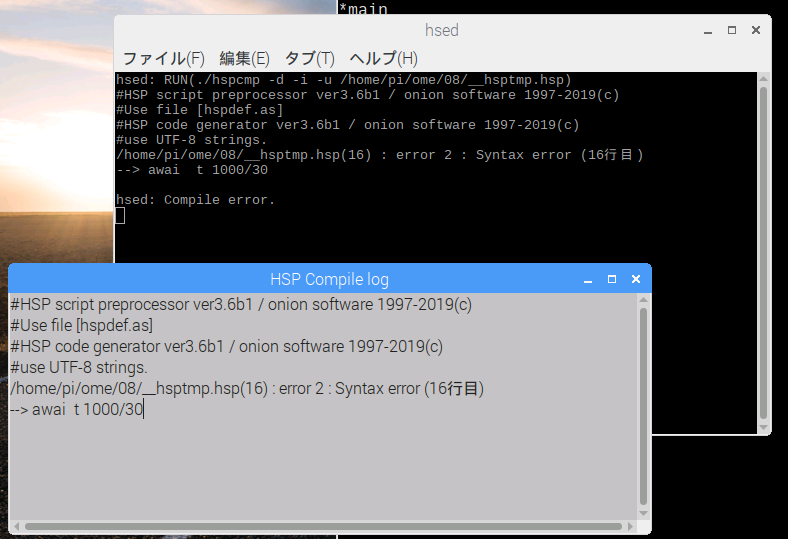
\includegraphics[keepaspectratio,width=11.324cm,height=7.756cm]{text04-img/text04-img011.png}
      \caption{エラーの表示}
    \end{center}
    \label{fig:prog_menu}
\end{figure}

エラーが発生した時は、エラーの内容と「(xx行目)」というエラーの場所が示されます。

エディタの左下に現在カーソルがある行番号が表示されているので、エラーの場所を見直してください。

わからない時は、先生かTAに質問してみましょう。

どうしても動かなくなってしまった時には、元になっているファイルが保存されているので、

「/usr/local/share/ome/04」フォルダ内の元のファイル(kick.hsp)をもう一度コピーして使ってみてください。